\chapter{Introduction}
The use of video-based surveillance system is nothing new. Over the past decade, both private and public sectors benefited from the ease of implementation along with the low implementation cost.
Retail stores, shopping malls, public places and private homes has equipped themselves with closed circuit television (CCTV) systems as a means for safety precaution.
With the rise of such technology and coupled with the hype around the introduction of Internet of Things (IoT), Big Data and even Industry 4.0 over the recent years, there has been a deeper thirst among researchers in finding practical use case by bridging existing data with technology to bring about a new wave in the research field.

\section{Research Overview}
\label{section:introduction}

The growth of the surveillance industry has also brought forth the rise of constant streams of video data. According to a research done by the IHS Markit (a leading source of information, insights and analytics) claimed that by 2019, the average data generated daily by new surveillance camera shipped globally will grow up to 2,500 petabytes daily \cite{woodhouse2016big}.
As you are reading, hundreds of thousand, if not millions of hours worth of video data are filling up database warehouses across the globe by the second. While these video footages are useful when it is needed (for example, when dealing with crime scene investigations), most of the time, these data are stored and left unprocessed, taking up additional storage space while compounding on the overhead cost.
This \textit{'reactive-approach'} towards surveillance systems makes it slow and difficult for investigators when dealing with crime scenes.

Looking from the another angle, the entertainment sector is also dishing out multimedia contents at a rather alarming rate. These digital contents are being pushed into data warehouses and consumed by the general public on a daily basis. General public as a whole has also benefited from the rise of various video search engines and tools such as Google, YouTube, Dailymotion and Bing. However, it is unlikely for these existing technologies to be directly applied towards surveillance video footages and excel in finding the desired footages. Nevertheless, it is clear that the idea of using search engines to retrieve video footage is nothing new. Hence, inspirations were drawn from these technologies and applied into the research problem at hand. %which will be discussed in this work.

All of the aforementioned retrieval engine technologies have one thing in common - the underlying concept. First, the process begins with extraction of video metadata such as title, description, filename, dates, subtitles and various other details that could assist in identifying these footage. Next, these videos are stored in the database along with the extracted metadata which can be used during the retrieval process. Finally, when a text-based query is issued, these video shots are retrieved and are then sorted in a way that best represents the query for the end users.
However, as mentioned, this approach can not be directly applied towards surveillance video footage as the metadata such as title, description or even tags does not exist most of the time.

Now, from the surveillance video footage standpoint, the traditional approach of finding a particular video from a huge collection is done manually. This process typically involves an inquirer/user who is searching for a particular scene or shot, and one of more person-in-charge who manages the video collection. Narrowing further down to the research topic, in a car-park surveillance setting, the inquirer would typically need to provide vehicle specific \textbf{semantics} such as time, date, colour of the vehicle, vehicle registration number, and place of which an incident occurred. %In this work, these information are examples of what would be referred to as semantics.

Next, the person-in-charge would have to sift through hours and hours of video in order to find potential video footages that matches the provided information. This \textit{'reactive-approach'} towards incidents is undeniably slow and ineffective. The entire process is time consuming, laborious and monotonous in nature. While the task is potentially straightforward when there is only one intended video shot with clear-cut definitive time and date given; this process takes enormous effort when details such as the time and date is not given, or even in cases when all the video shots with similar properties are desired within a given time period. Evidently, there exist a gap which can be addressed using a \textit{'proactive-approach'} via a well designed semantic extraction and retrieval techniques which this work attempts to address.

\section{Motivation, Problem Statements and Research Questions}

As described in the previous section, the traditional method used to retrieve desired surveillance video footages is not an effective use of time and manpower. In this section, the motivation to address the topic at hand is further discussed from the computer vision and natural viewpoint.

%explain what constitutes a good semantic extraction tool and a retrieval engine
%\subsection{Motivation}

At the frightening collection rate of surveillance video data, employing human labour to manually extract information from the video data source will undoubtedly be time consuming and be extremely labour intensive.
While not impossible, the simple act of watching the same scene over and over again from the video source will definitely put mental and physical strain on the task personnels. When considering the amount of legacy video data that has been collected over the years and the amount of insights it could offer, the time taken to analyse them manually would increases exponentially. Thus, affecting and foregoing the chance of reaping the benefits from these past data.

With the disadvantages of performing these task manually etched in mind, deployable computer vision techniques to extract information from video data could potentially alleviate the burden. In fact, the use of such techniques is not new, a generic Computer Vision task can be visualized using Figure \ref{fig:genericCV}. Works in regards to extracting vehicle-specific attributes can be found from the early 90's and it is still an ongoing research area. Viewing from a wider scope, a bulk of these research has placed their focus on \textit{highway} \cite{yu2017improved, cao2016vehicle, arya2016real, liu2016highway, al2016adaptive}, and  \textit{intersections} \cite{meng2017traffic, choong2017modeling, ren2018learning} datasets. Among the rare few \cite{shi2017study, marmol2016quickspot, ling2017identifying} that works on a car park dataset, the primary objective tend to revolve around the availability of parking spots.

\begin{figure}[!hbt]\centering

\includegraphics[width=.8\textwidth]{image/general/simpleframe.png}
\caption{Generic Computer Vision Task}
\label{fig:genericCV}
\end{figure}

The rise of technology has benefited researchers in the computer vision area greatly due to higher computational power at lower price points. The ability to churn out metadata from raw video footages quicker combined with the advantages of easily interpretable and meaningful semantics exhibits great commercial potential. Even so, there are still plenty of challenges and opportunities which are yet to be solved to improve on existing techniques. As mentioned in Section \ref{section:introduction}, existing popular video retrieval engines such as YouTube generally relies on keyword-based queries. Queries such as 'Selecting all vehicles entering from Entrance (A) and turning into Junction (B)' are ineffective as it may not capture the semantic content required by the end user.

Several authors attempted to solve this challenge by proposing the use of example-based queries \cite{zhang2017car, liu2016large, castanon2016retrieval} to facilitate the retrieval process.
These queries typically require end users to provide inputs in the form of an image or sample of the desired output. While it is possible to provide a thumbnail image-example for different scenes (e.g., beach, mountain, waterfall) and objects (e.g., bicycle, pen, lipstick), this is difficult with surveillance video footages as these data are often similar throughout the recorded duration. Plus, it would be highly unlikely for end users to have a copy of the sample footage.

In order to tackle this research problem, here are some research questions which will be addressed in this work:
\begin{enumerate}
\item What ideology and concepts can we glean from existing techniques and take advantage of them for the sake of the topic of interest?
\item How can we represent surveillance video footages in the form of semantics? What types of semantics can be extracted? How can these semantics be translated into something which is easily interpretable for the querying process?
\item How can we develop retrieval techniques that takes in input queries which are intuitive, flexible and user friendly while providing accurate search results in a sorted manner according to its relevance?
\end{enumerate}



\subsection{Research Objectives}
The objectives of this thesis can be divided into two main interdependent entities. As a whole, this work aims to adopt and leverage on existing frameworks to design objects semantics \textbf{extraction} and \textbf{retrieval} framework and techniques from \textbf{car park video footages}. In order to answer the research questions posed, the following objectives were set:

\begin{enumerate}
%\item To adopt and leverage on existing video data representation, semantics extraction and retrieval methods to design a surveillance video semantics extraction and retrieval framework.
  \item To identify and \textit{extract suitable semantics} which are easily interpretable while accurately describing car park surveillance events.
  \item To design \textit{video retrieval techniques} that takes in intuitive user-described queries to provide fast and accurate results.
\end{enumerate}

\subsection{Scope and Definition}
\label{subsec:scope}
The work in this thesis encompasses tasks found in a generic computer vision vehicle semantic extraction and retrieval framework as illustrated in Figure \ref{fig:framework}. The preliminary task of detecting, tracking and obtaining the \textit{bounding box} of each vehicle is assumed to be \textbf{obtained} prior to the semantic extraction task.
Hence, the task of \textit{extracting semantics} from the vehicles and the task of \textit{retrieving video footages} are the \textbf{central emphasis} in this work.
As most of the existing works only used a couple of hours/days in their dataset, in this work, the phrase \textbf{'long-term'} is used to refer to the duration (one month) of videos in which the vehicle semantics were extracted and retrieved from. Based on my study, the largest dataset in related works used up to 500 hours to count the number of different trajectories.


The scope of this work is further constrained to surveillance video footages taken from a \textit{single dataset}. This dataset contains videos captured from a single camera with a \textit{stationary viewpoint} (see Section \ref{section:dataset_used}). To further clarify the intent of this work, vehicle specific attributes are referred to as 'semantics'. This includes vehicle colour, trajectory, time and date of spotting the vehicle as well as location of vehicle in the scene. However, this does not include vehicle semantics such as vehicle brand, car segment (e.g.: sedan, hatchback, etc), and travelling speed. The extraction of scene semantics such as weather information, lighting condition and overall car park occupancy rate are also out of the scope of this work.


\subsection{Contribution}
As this thesis comprise of a collection framework, formulation of concepts and algorithms, the contribution of this work can be summarized as follow:


\begin{enumerate}
\item Designed a framework for the \textbf{extraction of vehicle specific semantics} which includes colour information of a vehicle throughout its tracked-life-cycle, the relative position of the vehicle at each frame, time and date information of when the vehicle was observed in the surveillance footages as well as size information of each vehicle. One of the proposed method employs an algorithm that averages out the dominant \textbf{colour} over the course of tracking it and ranking it against a set of eleven different hues. This is a challenging task as outdoor scenarios are often non-ideal due to its ever-changing illumination and weather conditions which would directly affect the classification accuracy of vehicle colours. The relative position of each vehicle was compiled into trajectory sets that represents the \textbf{motion} throughout the car-park. The time and date information for each vehicle are also extracted as these information are important in a surveillance scenario. To take advantage of the inherent property of video data, the spatio-temporal cube design was adopted to uniquely identify each section of the video footage.
\item Proposed two \textbf{video retrieval techniques} that takes in a trajectory input along with the colour, time and date semantics as the input. Unlike traditional retrieval engine that takes in known-keyword-based queries, this work proposed an unconventional yet intuitive trajectory input in the form of \textbf{user-described trajectory path} on the search canvas. Further, the colour, time and date semantics are given as keyword-based inputs for the retrieval engine to locate and rank video shots according to its similarity. As with any large scale retrieval engine, the collection of all the ground truth data is not a viable option. Therefore, the performance of the proposed method was tested against semantics extracted from one month's worth of data was measured and recorded using Precision@K and normalized Discounted Cumulative Gain metrics.
\end{enumerate}

\subsection{Organisation of Thesis}

The road-map of this thesis is laid out as follow: First, the introduction on the subject matter is discussed in this chapter.
In Chapter \ref{section:litreview}, first a brief overview of related theoretical background concepts is dicussed in Section \ref{subsec:relatedConcepts}. Then, in Section \ref{section:relatedworks}, related works in this research field are reviewed thoroughly to provide an understanding on what has been tried and solved, disadvantages along with potential areas of improvements that could be addressed.
In Chapter \ref{chapter:framework}, an overview of the proposed method's framework, dataset along with the experimental methodologies is described.
Chapter \ref{section:semanticsextraction} and Chapter \ref{section:retrievalengine} describes both the main components: i) \textbf{Semantics Extraction} and ii) \textbf{Semantics Retrieval}, however, the organization within these Chapters were divided into two cascaded phases.
Figure \ref{fig:proposedmethodoverview} illustrates these two phases.
Chapter \ref{section:semanticsextraction} focuses on the video semantics extraction methods for both the vehicle colour and vehicle motion, while Chapter \ref{section:retrievalengine} discusses the proposed retrival techniques along with the results and analysis.
Finally, the conclusion of this work along with potential future works is prepared in Chapter \ref{section:conclusion}.



\begin{figure}[!hbt]\centering
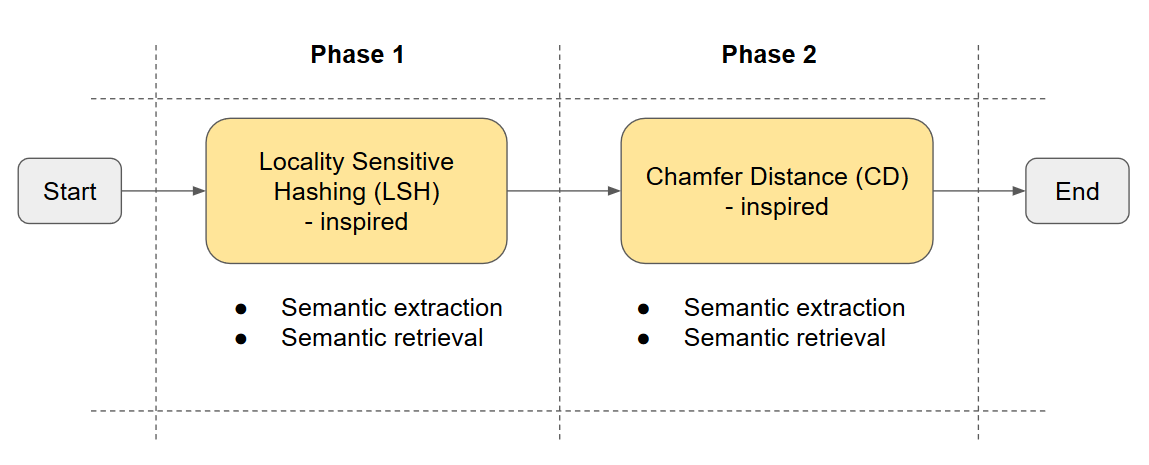
\includegraphics[width=\textwidth]{image/general/phases.PNG}
\caption{Proposed Method Overview}
\label{fig:proposedmethodoverview}
\end{figure}
